\documentclass[11pt,a4paper,oneside]{article}
\usepackage[utf8]{inputenc}
\usepackage{geometry}
 \geometry{
 a4paper,
 total={170mm,257mm},
 left=20mm,
 top=20mm,
 }
 \newcommand\independent{\protect\mathpalette{\protect\independenT}{\perp}}
\def\independenT#1#2{\mathrel{\rlap{$#1#2$}\mkern2mu{#1#2}}}
\usepackage{amsmath}
\usepackage{amsfonts}
\usepackage{amssymb}
\usepackage{graphicx}
\usepackage{color}
\usepackage{subfigure}


\author{Mohamed-El-Amine Seddik \hspace*{2em} Marwen Sallem \hspace*{2em} Kais Slimi \hspace*{2em} Oussama Bouraoui}
\title{ML Project : Machine Learning Methods Applied to Human Physical Activity Classification Using On-Body Sensors}
\begin{document}
\maketitle
\begin{abstract}
This paper describes our choice for the machine learning project subject, we chose to work on applying machine learning methods to the problem of human physical activity classification, based on data that comes from on-body sensors. Basically, the aim of this project is to explore different techniques of machine learning and to apply them to this particular problem.
\end{abstract}
\section*{Motivation}
The ability of designing a system that automatically classifies the physical activity performed by a given person is very attractive for many applications in various fields such that health-care monitoring and in developing smart human-machine interfaces. There are several techniques to handle this task, and mainly some of them are based on computer vision where some others aims to use on-body sensors. Based on \cite{mannini} we chose to work on data that comes from on-body sensors. In fact, there is many datasets available on the internet that are used for this special problem, we provide below a link to a dataset that we plan to use for our project. 
\section*{Goal}
As illustrated by the title, our main goal is to classify the Human Physical Activity. To reach this goal we plan to explore different machine learning methods (Probabilistic based methods like HMM and geometric based ones as SVM k-NN ...) and to apply them to this particular task, at the end we aim to provide the performances of the different applied methods.
\section*{Dataset}
- https://archive.ics.uci.edu/ml/datasets/Activity+Recognition+from+Single+Chest-Mounted+Accelerometer

\newpage

\section*{Introduction}

Several techniques have been used to recognize Human activities such as video-based sensors, wearable-based sensors, environmental sensors and object sensors like smart phones. In this paper, wearable-sensors based systems for activity recognition has been used. 

Human activity recognition or (HAR), begins by collecting the raw data from sensors worn on certain parts of the body. The sensors will provide different data depending on the part of the body where it’s worn (for example wrist, chest, \ldots) and the technical characteristics of the sensor itself. One of the biggest challenges of HAR is to overcome this variability in sensor characteristics. The sensors usually have limited processing power which makes it difficult to get a high frequency sampling or do any kind of preprocessing on the sensors.\cite{bulling}

We are therefore unable to use the raw data directly for the classification task. We need to do several preprocessing steps depending on the classification method we want to use. In section \ref{pre} we will explain the state of the art feature extraction techniques encountred in such problems.

Another issue in HAR is Intraclass variability: Different people will do the same activity differently. Their data on the sensors will not be very similar but it will have the same label (in the supervised setting) or the classifier has to assign them the same label (in the unsupervised setting). This can be overcomed by collecting more data or develop person-independant features that are more robust to this variability. In the section \ref{kda}, we will present a supervised technique that aims to classsify the human activities using LDA and KDA classifier. But generally the supervised approaches require a large amount of labelled data. They are too expensive. For that, one has to rely on unsupervised approaches. Hence, we will present in \ref{hmm} an unsupervized technique  based upon joint segmentation of multidimensional time series using a Hidden Markov Model (HMM) in a multiple regression context and is denoted by MHMMR: Multiple Hidden Markov Model Regression.

%  Both sections \ref{kda} and \ref{hmm} will present two methods that are used to overcome this problems.

% To recognize human activities from on-body wearable accelerometers, there are two appraches: supervised and unsupervised machine learning. Generally the supervised approaches require a large amount of labelled data. 
% They are too expensive. For that, one has to rely on unsupervised approaches. This paper presents a new unsupervised approach for human activity recognition from raw acceleration data measured using inertial wearable sensors. 

\section{Pre-processing and features extraction}
\label{pre}
Acclerometers provide three axis time series $A_x$, $A_y$ and $A_z$. Once sampling on a known frequency, we obtain a different signal for each class, for instance the figure \ref{fig-signals}

\begin{figure}[ht!]
\begin{center}
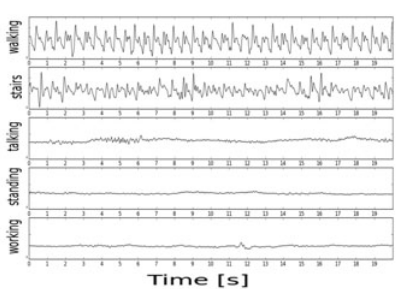
\includegraphics[scale=.7]{signals}
\caption{Accelerometer Data for Five Different Activities \cite{mannini}}
\label{fig-signals}
\end{center}
\end{figure}
To be able to apply Machine Learning techniques, we have to extract features from these given signals. These latter is mainly done on two different phases :

In the first phase we are going to widen our signal databases by adding new signals :
\begin{itemize}

\item We will compute the magnitude of the acceleration : $A_m = \sqrt{A_x^2 + A_y^2 + A_z^2}$ \cite{casale}. 
\item We will separate every axis time-series in high-frequency (AC) components that captures dynamic motion, and low-frequency (DC) components related to the gravity's influence that captures static postures.  	Thereby, we will obtain for each time series three additional time series that corresponds to the signal without filtering, the signal after applying a high-pass filter and the signal after applying a low-pass filter.
\end{itemize}

Now we have 12 signals extracted from the three initial signals $A_x$, $A_y$ and $A_z$. Having these new set of signals, we will split them into some windows in order to compute features. In fact, we apply a windowing and overlapping process which means that we will take windows of 52 sample (1 second of data) with 50\% of overlapping between windows. Thus, we can move to the second phase, i.e extracting features :

\begin{itemize}
\item  We compute the RMS of the velocity (integration of acceleration) and mean value of Minmax sums\footnote{The Minmax sums are computed as the sum of all the differences of the ordered pairs of the peaks of the time series.\cite{casale}}  . In \cite{casale} we showed that theses features are the most important for the proposed Random Forest classifier in the Table \ref{fig-table}.

\item Basic statistics as mean value, standard deviation, skewness, kurtosis, correlation between each pairwise of accelerometer axis. In fact, Manini and Sabatini shows in \cite{mannini} that  these features proved to be useful in HAR.

\item Other features like ARIMA coefficients \cite{mannini} and energy of the coefficients of some level wavelet decomposition \cite{casale} are also of great importance.
\end{itemize}

\begin{figure}[ht!]
\begin{center}
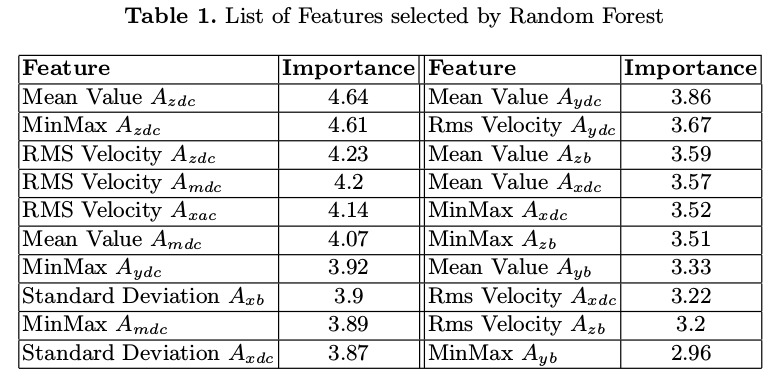
\includegraphics[scale=.5]{table}
\label{fig-table}
\end{center}
\end{figure}
Now, we will have more than 300 features. It's possible to use them either in Single-Frame approaches as " Linear and Kernel Discriminant Analysis approaches " or in Sequential approaches like " Hidden Markov Model Regression " which we will describe in the next two sections. 


\section{Linear and Kernel Discriminant Analysis approaches}
\label{kda}
One observes the raw data of the chosen dataset, we acknowledge an overlapping between the different classes (see Fig~\ref{fig:first}), this overlapping is due to the high with-in and low between-class variances. Based on \cite{khan}, in order to fix this overlapping problem, we present in this section the LDA and KDA models, which are a supervised classification approaches that utilizes the class specific information maximizing the ratio of the within and between class scatter information. In particular, the KDA is a generalization of LDA applied in a RKHS feature space.

\begin{figure}[ht!]
\begin{center}
\subfigure[Raw data plotted for different classes.]{
\label{fig:first}
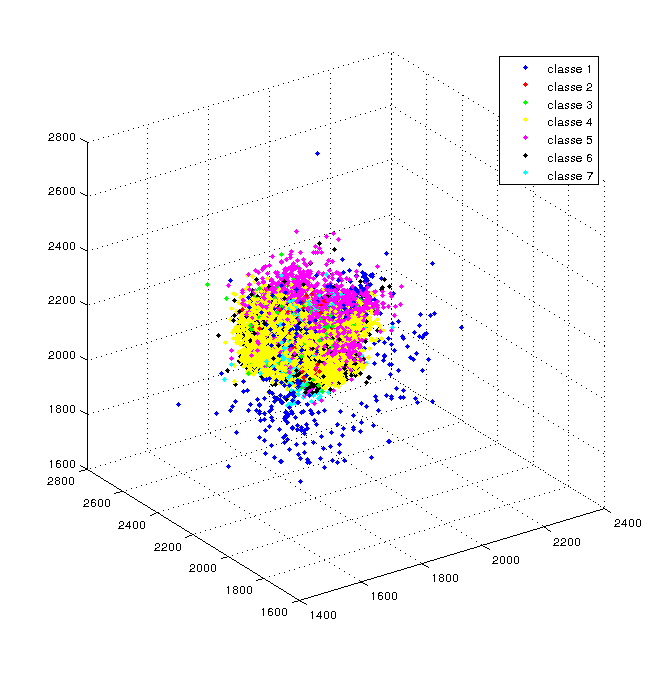
\includegraphics[scale=.3]{classes}
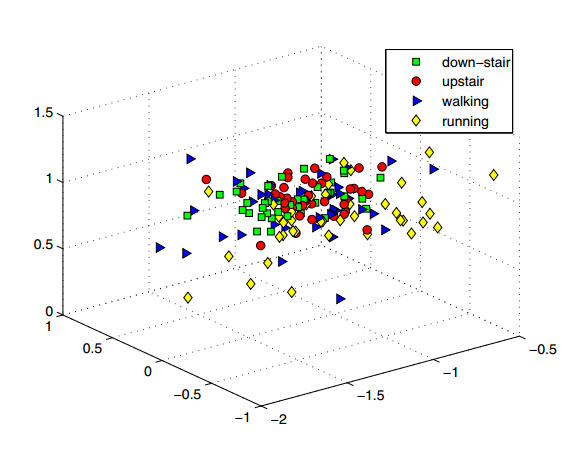
\includegraphics[scale=.3]{a}}

\subfigure[Results of applying LDA (left) and KDA (right) to the raw data.]{
\label{fig:second}
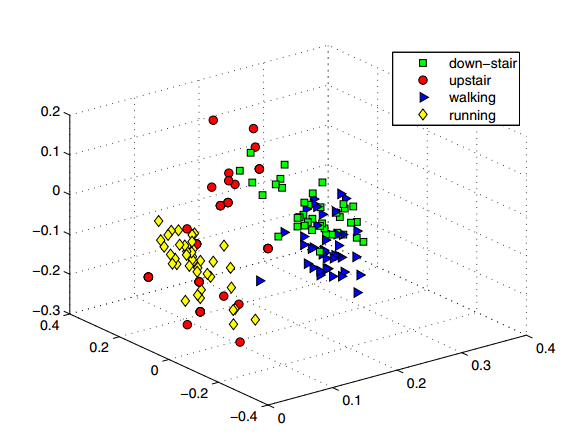
\includegraphics[scale=.3]{b}
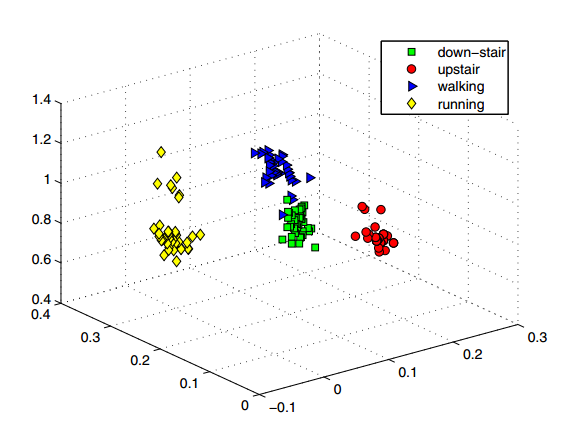
\includegraphics[scale=.3]{c}}
\end{center}
\caption{Visualization of the different classes before and after applying Linear and Kernel Discriminant Analysis, we notice that the classes are perfectly separable ones applying the KDA (see \ref{fig:second} right).}
\end{figure}

\subsection{Theory about Linear Discriminant Analysis}
The LDA responds to the question of how do we use the label information in finding informative projections of our data? To that purpose it considers maximizing the following objective:
\begin{equation}
(\mathcal{P}):\quad \max_{\omega} J(\omega) = \max_{\omega} \frac{\omega^T S_B \omega}{\omega^T S_W \omega}
\end{equation}
Where $S_B$ is the between classes scatter matrix and $S_W$ is the within classes scatter matrix. And are given by:

\begin{equation}
S_B = \sum_c (\mu_c - \bar{x})(\mu_c - \bar{x})^T \quad S_W = \sum_c \sum_{i\in c} (x_i - \mu_c)(x_i - \mu_c)^T
\end{equation}
Where $\bar{x}$ overall mean of the data.\\
$J$ being invariant with respect to re-scaling of the vector $\omega \rightarrow \alpha \omega$. Thus we can always choose $\omega$ such that $\omega^T S_W \omega=1$, so that the problem ($\mathcal{P}$) could be written as:
\begin{equation}
(\mathcal{P}):\quad \min_{\omega} -\frac{1}{2} \omega^T S_B \omega \texttt{ s.t. } \omega^T S_W \omega =1
\end{equation}
The Laplacian of ($\mathcal{P}$) is thus:
\begin{equation}
\mathcal{L}_{\mathcal{P}}(\omega,\lambda) =  -\frac{1}{2} \omega^T S_B \omega + \frac{1}{2} \lambda (\omega^T S_W \omega-1)
\end{equation}
Finally, taking the derivative with respect to $\omega$ of the Laplacian, one get:
\begin{equation}
S_B \omega = \lambda S_W \omega \Rightarrow S_W^{-1} S_B \omega = \lambda \omega
\end{equation}
$S_B$ is symmetric positive definite (p.d.), thus $S_B = S_B^{1/2}S_B^{1/2}$ where $S_B^{1/2} = U \Lambda^{1/2} U^T$ (where $U \Lambda U^T$ is the eigen-decomposition of $S_B$). So performing the change of variable $v=S_B^{1/2} \omega$, one get:
\begin{equation}
\underbrace{S_B^{1/2} S_W^{-1} S_B^{1/2}}_{\texttt{symmetric p.d.}} v = \lambda v
\label{eigen}
\end{equation}
Finally, the goal of the LDA is to find the eigenvector corresponding to the largest eigenvalue of the symmetric p.d. matrix $S_B^{1/2} S_W^{-1} S_B^{1/2}$. Denote this vector $v^*$, thus $w^* = S_B^{-1/2}v^*$.

\subsection{Theory about Kernel Discriminant Analysis}
To kernelize the LDA, we consider the problem in a feature space $\mathcal{F}$ induced by some non-linear mapping function $\phi : \mathbb{R}^d \rightarrow \mathcal{F}$. An inner product $<.|.>_{\mathcal{F}}$ can be defined in $\mathcal{F}$ which makes for so called reproducing the kernel Hilbert Space (RKHS). More precisely $<\phi(x_i)|\phi(x_j)>_{\mathcal{F}}=K(x_i,x_j)$ holds where $K(.,.)$ is a p.s.d. kernel function. Thus, to find the linear discriminant in $\mathcal{F}$, we need to maximize:
\begin{equation}
(\mathcal{P}_K):\quad \max_{\alpha} J_{\phi}(\alpha) = \max_{\alpha} \frac{\alpha^T S_b^{\phi} \alpha}{\alpha^T S_w^{\phi} \alpha}
\end{equation}
Where 
\begin{equation}
\begin{split}
S_b^{\phi} = \sum_c n_c (K_c K_c^T - K K^T)\\
S_w^{\phi} = K^2 - \sum_c n_c K_c K_c^T \\
K_c = \frac{1}{n_c} \sum_{i\in c} K_{i,j}, \quad K = \frac{1}{n} \sum_{i} K_{i,j}
\end{split}
\end{equation}
According to the equation (\ref{eigen}), one get the $\alpha$ which maximizes the objective above, denote by $\alpha^*$ this solution. Thus, $\omega_*$ in the initial space is given by:
\begin{equation}
\omega_* = \sum_i \alpha_i^* \phi(x_i)
\end{equation}
And finally using the kernel trick, we don't need to compute explicitly $\phi$, and the projection of a new sample $x$ over $\omega_*$ is given by:
\begin{equation}
\omega_*^T\phi(x) = \sum_i \alpha_i^* K(x_i,x)
\end{equation}



\section{An Unsupervised Approach for Automatic Activity Recognition based on Hidden Markov Model Regression \cite{attal}}
\label{hmm}

In the proposed model, each activity is represented by a regression model and the switching from one activity to another is governed by a hidden Markov chain.
The MHMMR parameters are learned in an unsupervised way from unlabelled raw acceleration data acquired during human activities using the Expectation-Maximization (EM) algorithm where no activity labels are needed. 

The acceleration data are presented as multidimensional time series presenting various regime changes. In such context, the goal is to provide an automatic partition of the data into different segments (regimes),each segment being considered afterwards as an activity. \ \\

In Hidden Markov Model Regression (HMMR), each time series is represented as a sequence of observed univariate variables $(y_1, y_2, \ldots , y_n)$, where the observation $y_i$ at time $t_i$ is assumed to be generated by the following regression model: 

\begin{equation}
y_i = \beta_{z_i} + \sigma_{z_t}\epsilon_i \text{ ; } \epsilon_i \sim \mathcal{N}(0,1)  \text{ , } (i = 1, \ldots, n) 
\end{equation}

% \begin{figure} [h!]
% 	\begin{center}
% 		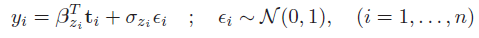
\includegraphics[scale=0.8]{1.png}
% 	\end{center}
% \end{figure}

where $z_i \in (1, \ldots ,K) $ is a hidden discrete-valued variable. In this application case, $z_i$ represents the hidden class label (activity) of each acceleration data point and $K$ corresponds to the number of considered activities. The variable $z_i$ controls the switching from one polynomial regression model associated to one activity, to another of $K$ models at time $t_i$. 

The HMMR assumes that the hidden sequence $ z = (z_1, \ldots, z_n)$ is a homogeneous Markov chain of first order parameterized by the initial state distribution $\pi$ and the transition matrix $A$. Regarding the multiple regression case, the model can be formulated as follows:

\begin{eqnarray}
y_i^{(1)} & = & \beta^{(1)T}_{z_i} + \sigma_{z_t}^{(1)} \epsilon_i \\
y_i^{(2)} & = & \beta^{(2)T}_{z_i} + \sigma_{z_t}^{(2)} \epsilon_i \\
\vdots & & \vdots \\
y_i^{(d)} & = & \beta^{(d)T}_{z_i} + \sigma_{z_t}^{(d)} \epsilon_i \\
\end{eqnarray}

% \begin{figure} [h!]
% 	\begin{center}
% 		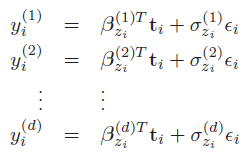
\includegraphics[scale=0.8]{2.png}
% 	\end{center}
% \end{figure}

where $d$ represents the dimension of the time series.

The Multiple HMMR model is therefore fully parameterized by the parameter vector :
\begin{equation}
\theta = (\pi,A,B_1, \ldots,B_k, \Sigma_1, \ldots ,\Sigma_k)
\end{equation}

where $B_k$ is the matrix of the multiple regression model parameters associated with the regime (class) $z_i = k$ and $\Sigma$ its corresponding covariance matrix. 

The parameters are estimated by maximizing the observed data likelihood through the Expectation-Maximization (EM) algorithm. The log-likelihood to be maximized in this case is written as follows: 

\begin{equation}
\mathcal{L}(\theta) = \log p(y_1, \ldots, y_n; \theta) = \log \sum_z p(z_1;\pi) \prod_{i=2}^n p(z_i|z_{i-1};A) \prod_{i=1}^n \mathcal{N}(y_i; B_{z_i}^T, t_i, \Sigma_{z_i})
\end{equation}

% \begin{figure} [h!]
% 	\begin{center}
% 		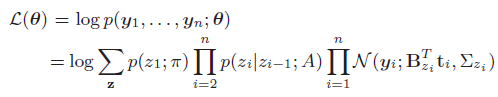
\includegraphics[scale=0.8]{3.png}
% 	\end{center}
% \end{figure}

To evaluate the performence of this method, it has to be compared to other algorithms. Compared to standard unsupervised classifiers, the proposed MHMMR outperforms them since it provides the best classification rate, $91.4\%$. 

\begin{figure} [h!]
	\begin{center}
		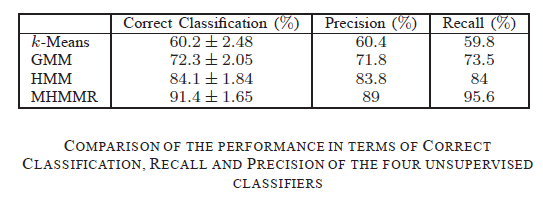
\includegraphics[scale=0.8]{4.png}
	\end{center}
\end{figure}

For the supervised learning, the k-NN $(k = 1)$ gives the highest classification rates with $95.8\%$, followed by the Random Forest with $93.5\%$.

\begin{figure} [h!]
	\begin{center}
		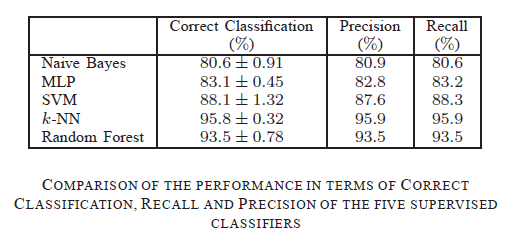
\includegraphics[scale=0.8]{5.png}
	\end{center}
\end{figure}





% \section*{References}
% \ \\

% [1] Mannini, A. Sabatini, A.M.	Machine Learning Methods for Classifying Human Physical Activity from On-Body Accelerometers. Sensors 2010, 10, 1154-1175.\ \\ 

% [2] D. Trabelsi, S. Mohammed, F. Chamroukhi, L. Oukhellou, and Y. Amirat, IEEE Transactions on Automation Science and Engineering, Volume: 10, Issue: 3, July 2013, Pages: 829-835.\ \\

% [3] A. M. Khan, Y. K. Lee, S. Y. Lee and T. S. Kim, "Human Activity Recognition via an Accelerometer-Enabled-Smartphone Using Kernel Discriminant Analysis," 2010 5th International Conference on Future Information Technology, Busan, 2010, pp. 1-6.
% doi: 10.1109/FUTURETECH.2010.5482729

\bibliographystyle{unsrt}
\bibliography{biblio.bib}


\end{document}